\section{Buffer is becoming extremely\\ shallow}\label{sec:background}
\vspace{-1mm}
In this section, we first understand the buffering logic of existing chips. Then, we quantify the buffer requirements of TCP\footnote{In this paper, by TCP we refer to various TCP-variants, such as DCTCP~\cite{dctcp} and ECN$^{*}$~\cite{tuning}, \etc, that are designed for datacenters.} at high-speed. Finally, we show that the buffer space becomes increasingly insufficient as link speed increases.

\subsection{Understanding the switch buffering}
On the switching chip, the Memory Memory Management Unit (MMU) allocates the on chip buffer memory to incoming packets. The buffer memory is divided into several pools, which can be classified into following two categories:
\begin{ecompact}
\item \textbf{Private Pools:} dedicated buffers reserved to egress queues.
\item \textbf{Shared Pools:} shared buffers that can be used once the destination egress queue's private pool has been used up.
\end{ecompact}

When a packet arrives, the MMU first tries to enqueue it into the private pool of the destination queue. If there is no enough buffer space, the MMU tries to enqueue it into the shared pool. The packet only gets dropped by MMU if neither the private pool nor the shared pool has enough space. Moreover, the MMU only drops new arriving packets. Packets in the pool cannot be pushed out and dropped.

\subsection{Buffer requirement of TCP at high-speed}\label{subsec:buffer_requirement_high_speed}
TCP is the dominant transport protocol in DCNs~\cite{dctcp}. The switch buffer is crucial for TCP's performance. Moderate buffer occupancies are necessary for high throughput~\cite{sizing}. Futhermore, we also need some buffer headroom to absorb transient busrts~\cite{dctcp}. Therefore, insufficient switch buffers cause (1) \textbf{low throughput}, thus slowing bulk transfers and (2) \textbf{excessive packet losses}, thus resulting in large tail completion times for small messages.

To achieve the desired performance, TCP requires \emph{at least} $C\times RTT \times \lambda$ buffer space per port, where $C$ is the link capacity, $RTT$ is the average round-trip time and $\lambda$ is a characteristic constant of the congestion control algorithm\footnote{Due to the small number of concurrent large flows in DCNs~\cite{dctcp}, we can assume large flows are synchronized here.}. In recent years, the link speed in DCNs has increased greatly, from 1Gbps to 40Gbps and now to 100Gbps. However, the base latency does not change much as it is mainly determined by processing overhead introduced by various sources (\eg, kernel network stack, driver, NIC and middlebox) along the path. Hence, the buffer demand of TCP almost increases in proportion to the link speed in DCNs.

\vspace{-1mm}
\parab{Testbed measurement:}In out testbed, three servers (Mellanox ConnectX-4 100Gbps NIC, Linux kernel 3.10.0) are connected to a Arista 7060CX-32S-F switch. The base latency in is $\sim$30$\mu$s. We consider two TCP variants: DCTCP~\cite{dctcp} and ECN$^{*}$~\cite{tuning} (regular ECN-enabled TCP which simply cuts window by half in the presence of an ECN mark). We generate 16 long-lived flows using \texttt{iperf} from two senders to a receiver. We vary the RED marking threshold\footnote{We set the maximum and minimum queue length thresholds of RED~\cite{RED} to the same value as previous work~\cite{dctcp,tuning} suggests.} and measure the aggregate throughput at the receiver side. For a TCP variant, its basic buffer requirement approximately equals to the minimum marking threshold delivering 100\% link utilization.

\begin{figure}[t]
\centering
  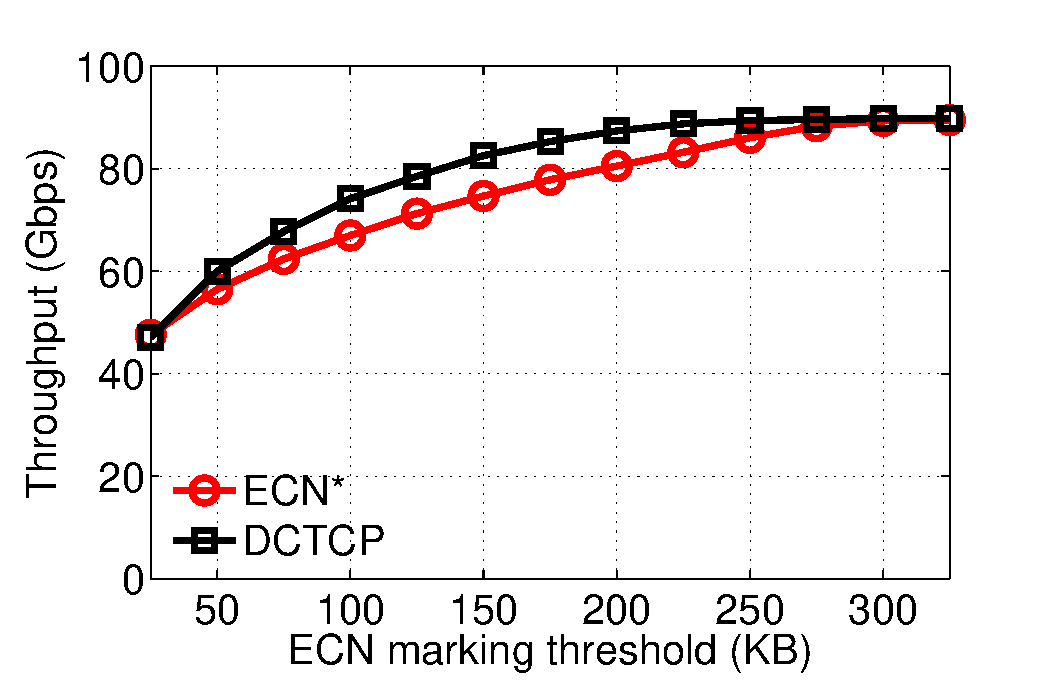
\includegraphics[width=0.75\linewidth]{figs/throughput_ecn_threshold.eps}
      \vspace{-1.5mm}
  \caption{[Testbed] Aggregate TCP throughput with different ECN/RED marking thresholds}\label{fig:throughput_ecn_thresh}
    \vspace{-4mm}
\end{figure}
\begin{table*}[t]
\small
\centering
\begin{tabular}{|l|l|l|l|l|}
\hline
ASIC & Broadcom 56538 & Broadcom Trident+ & Broadcom Trident \uppercase\expandafter{\romannumeral2} & Broadcom Tomahawk \\\hline
Capacity (ports $\times$ BW) & 48 p $\times$ 1 Gbps & 48 p $\times$ 10 Gbps & 32 p $\times$ 40 Gbps & 32 p $\times$ 100 Gbps \\\hline
Total buffer             & 4MB   & 9MB  & 12MB & 16MB (4 MMUs) \\\hline
Buffer per port          & 85KB  & 192KB  & 384KB & 512KB \\\hline
Buffer per port per Gbps & 85KB  & 19.2KB & 9.6KB & 5.12KB \\\hline
\end{tabular}
%\vspace{-2mm}
\caption{Information of some commodity datacenter switching chips. Note that Tomahawk has 4 switch cores, each with its own MMU and 4MB buffer~\cite{tomahawk_buffer1,tomahawk_buffer2}. Dynamic buffer sharing only happens within the single core.}
\label{tab:chip_buffer}
\vspace{-2mm}
\end{table*}
Figure~\ref{fig:throughput_ecn_thresh} shows aggregate throughput results with different thresholds.
As expected, ECN$^{*}$ starts to achieve 100\% throughput on 325KB which is close to the bandwidth-delay product (BDP) in our testbed. Our measurement also shows that DCTCP performs similar as ECN$^{*}$ in practice. The minimum ECN marking threshold that DCTCP requires for 100\% throughput is 250KB. The reader may be curious that why our experiment observation of DCTCP seems inconsistent with theory results in~\cite{dctcp-analysis} (0.17BDP buffering is enough for 100\% throughput). We think this is mainly due to packet bursts that are caused by various interactions between the OS and the NIC (\eg, TSO, GRO and interrupt moderation). Hence, a much larger ECN marking threshold is required to absorb bursts. Such complex burst behaviors are difficult to capture by ideal fluid model in~\cite{dctcp-analysis}, thus resulting in the theory-practice gap\footnote{Such performance-theory gap has also been identified by previous work~\cite{tuning} and even DCTCP paper itself~\cite{dctcp}.}. We also conduct the above experiment using Windows Server 2012 R2 and observe that DCTCP requires $\sim$60-70\% BDP buffering for 100\% throughput.

\vspace{-1mm}
\parab{Production Datacenters:}Compared to our simple small-scale testbed, production datacenters are more challenging and have larger base latency. At the end host, packets may experience high processing delay due to kernel scheduling. In the network, packets experience innegligible processing delay when going through various middleboxes (\eg, firewall, IPSec gateway and load balancer). Long-distance cables and multiple switch hops also bring several-microsecond delay. Above factors greatly increase the actual latency in production environments. In~\cite{pingmesh}, the authors show that even the 50th percentile inter-pod latency can exceed 200$\mu$s. Such latency eventually transfers to a large buffer demand. Consider a 100Gbps network with 80$\mu$s base RTT, the per-port buffer requirement of ECN$^{*}$ can easily reach 1MB.

\subsection{Buffer becomes increasingly insufficient}\label{sec:buffersize}
However, the buffer size of commodity switching chips does not increase as expected. We list buffer and capacity information of some commodity chips in Table~\ref{tab:chip_buffer}. The capacity significantly outpaces the buffer size, resulting in decreasing buffer per port per Gbps (from 85KB to 5.12KB). The reasons of shallow switch buffers are at least two-fold.
\begin{ecompact}
\item The memory used in switch buffers is high-speed SRAM. Compared to DRAM, SRAM is more expensive as it requires more transistors.
\vspace{-1mm}
\item The area increases with the memory size. When the area becomes large, the read/write latency will increase, making the memory access speed hard to match the link speed.
\end{ecompact}
Therefore, most commodity switches in DCNs are shallow buffered. We envision that such trend will hold for future 200/400Gbps switching chips.
